\documentclass{jcst}

% Required packages beyond jcst.cls defaults
\usepackage{booktabs}
\usepackage{multirow}
\usepackage{amsmath}
\usepackage{graphicx}
\usepackage{url}
\usepackage[spanish,english]{babel}
\usepackage{pgfplots}
\usepackage{tikz}
\usetikzlibrary{shapes.geometric, arrows, positioning}
\pgfplotsset{compat=1.18}
\usepackage{tabularx}
\usepackage{xcolor}

\sloppy
\hyphenpenalty=1000
\setlength{\emergencystretch}{3em}

% -------------------------------------------------------
%  TITLE — English + Spanish (required by JCST)
% -------------------------------------------------------
\title{Hierarchical Uncertainty Quantification for Reliable Automated Radiology Report Generation \\
\large Cuantificaci\'{o}n de Incertidumbre Jer\'{a}rquica para la Generaci\'{o}n Confiable
de Informes Radiol\'{o}gicos Automatizados}

% -------------------------------------------------------
%  AUTHORS
% -------------------------------------------------------
\author[1\orcid{0000-0001-2345-6789}]{Abdul Samad}
\author[1\orcid{0000-0002-3456-7890}]{Zain Ali}
\author[1\orcid{0000-0003-4567-8901}]{Ali Haider}

\affil[1]{School of IT, Institute of Management Sciences (IMSciences), Peshawar, Pakistan \authorcr
\{bsse.243203624, bsse.243205234\}@imsciences.edu.pk \quad ali.haider@imsciences.edu.pk}

% -------------------------------------------------------
\begin{document}
\selectlanguage{english}
\maketitle

% -------------------------------------------------------
%  ABSTRACT (English)
% -------------------------------------------------------
\begin{abstract}
With thousands of chest X-rays processed daily at facilities such as Khyber Teaching Hospital
(KTH) and Lady Reading Hospital (LRH) in low-resource areas like Khyber Pakhtunkhwa,
Pakistan, automated radiology report generation holds transformative potential for over-extended
diagnostic services. Deep-learning vision-language models currently produce reports
deterministically, without confidence scores, which can endanger patient safety through
hallucinated clinical findings. This paper introduces a three-level hierarchical uncertainty
quantification (UQ) framework that assigns calibrated confidence scores at word, sentence, and
section granularity. The architecture combines a Vision Transformer (ViT-Base/16) visual
encoder with a GPT-2 language decoder and stochastic inference via Monte Carlo (MC) Dropout.
Trained and evaluated on three publicly available Kaggle Chest X-ray datasets (combined
$n=5{,}863$ images), the system achieves BLEU-4 of 0.378 and CIDEr of 0.672, and correctly
identifies over 94.3\% of erroneous clinical statements at a safety threshold of $\tau=0.75$.
The Area Under the Calibration Error curve (AUCE) is 0.042, indicating strong probabilistic
calibration. Results confirm that hierarchical uncertainty estimation can be integrated into
automated radiology pipelines without degrading linguistic performance, providing a viable
pathway toward trustworthy AI-assisted diagnosis in under-resourced hospitals across Peshawar
and beyond.
\end{abstract}

\keywords{automated radiology report generation, chest X-ray, deep learning, Monte Carlo
Dropout, uncertainty quantification, Vision Transformer}

% -------------------------------------------------------
%  RESUMEN (Spanish — required by JCST)
% -------------------------------------------------------
\selectlanguage{spanish}
\renewcommand{\abstractname}{Resumen}
\begin{abstract}
Con miles de radiograf\'{i}as de t\'{o}rax procesadas diariamente en centros como el Hospital
Universitario de Jaiber (KTH) y el Hospital Lady Reading (LRH) en zonas de bajos recursos
como Jaiber Pajtunjwa, Pakist\'{a}n, la generaci\'{o}n autom\'{a}tica de informes radiol\'{o}gicos
tiene un potencial transformador para los servicios de diagn\'{o}stico sobrecargados. Los modelos
de visi\'{o}n-lenguaje actuales producen informes de manera determin\'{i}stica, sin puntuaciones
de confianza, lo que puede comprometer la seguridad del paciente mediante hallazgos cl\'{i}nicos
alucinados. Este art\'{i}culo introduce un marco de cuantificaci\'{o}n de incertidumbre (UQ)
jer\'{a}rquico de tres niveles que asigna puntuaciones de confianza calibradas a nivel de
palabra, oraci\'{o}n y secci\'{o}n. La arquitectura combina un codificador visual Vision
Transformer (ViT-Base/16) con un decodificador de lenguaje GPT-2 e inferencia estoc\'{a}stica
mediante Monte Carlo Dropout. El sistema logra un BLEU-4 de 0,378 y un CIDEr de 0,672,
e identifica correctamente m\'{a}s del 94,3\% de los enunciados cl\'{i}nicos err\'{o}neos con
un umbral de seguridad de $\tau=0,75$, con una curva AUCE de 0,042.
\end{abstract}

\palabrasclaves{aprendizaje profundo, cuantificaci\'{o}n de incertidumbre, generaci\'{o}n
autom\'{a}tica de informes radiol\'{o}gicos, Monte Carlo Dropout, radiograf\'{i}a de t\'{o}rax,
Vision Transformer}

\selectlanguage{english}

% ================================================================
\section{Introduction}
% ================================================================

Medical imaging diagnosis is one of the most cognitively demanding tasks in health care.
Radiologists must analyze chest X-rays, CT scans, and MRI images, then produce structured
reports that guide clinical decision-making. The worldwide deficit of radiologists has become a
critical problem: the physician-to-population ratio falls as low as one radiologist per 50,000
inhabitants in many developing countries, including Pakistan~\cite{who2023}.

Referral hospitals such as Khyber Teaching Hospital (KTH) and Lady Reading Hospital (LRH)
in Peshawar each receive 1,200--1,800 chest X-rays per working day with fewer than eight
radiologists on staff, causing diagnostic queues that delay treatment and worsen outcomes~\cite{kmu2022}.

Since the early 2010s, automated radiology report generation has been continuously
investigated. Retrieval-based approaches matched query images to pre-written templates~\cite{shin2016}.
More recently, end-to-end encoder-decoder networks have demonstrated strong performance: Chen
et al.\ introduced R2Gen, a memory-driven Transformer that set benchmark BLEU scores on
IU-X-Ray and MIMIC-CXR~\cite{chen2020}. Subsequent work incorporated medical knowledge
graphs~\cite{zhang2020}, cross-modal attention mechanisms~\cite{wang2021cross}, multi-scale
visual features~\cite{li2021}, and keyword-driven decoders~\cite{yang2021}. However, a
fundamental limitation persists across nearly all published systems: they are \emph{deterministic}.
A single point-estimate report is produced per image, with no measure of output reliability or
trustworthiness.

This property is clinically hazardous. When a clinician relies on an automated summary, a model
that \emph{hallucinate} a finding---presenting an erroneous clinical statement as if factual---can
mislead diagnosis~\cite{balachandran2022}. Uncertainty quantification (UQ) provides a
principled mechanism to associate confidence scores with model predictions, enabling downstream
systems and human reviewers to flag low-confidence outputs for expert scrutiny~\cite{gal2016,lakshminarayanan2017}.

Existing UQ methods applied to medical report generation remain coarse-grained. MC
Dropout~\cite{gal2016} or deep ensembles~\cite{lakshminarayanan2017} yield a single
report-level uncertainty score. These aggregate measures fail to localise the precise words or
sentences that drive overall uncertainty---a granularity required for clinical utility, where a
radiologist must be able to re-examine a specific passage rather than the report as a whole~\cite{shelmanov2021}.

This paper addresses that gap by proposing a hierarchical UQ framework that cascades confidence
signals across three granularity levels: word, sentence, and section. The four key contributions are:

\begin{enumerate}
  \item A hierarchical confidence-scoring framework computing normalised Shannon entropy at the
        token level and aggregating it upward to sentence and section level within structured radiology reports.
  \item Systematic calibration evaluation using AUCE, complemented by a safety-precision metric
        quantifying the false-positive rate of the confidence-scoring system for flagged uncertain tokens.
  \item Demonstrated performance on three Kaggle Chest X-Ray datasets compared against
        deterministic baselines, with actionable uncertainty signals.
  \item A deployment blueprint for a structured radiology report system in the low-resource
        clinical environment of Peshawar, enabling automatic approval of high-confidence report
        sections and expert-level review only for uncertain sections at KTH.
\end{enumerate}

The remainder of this paper is organised as follows. Section~\ref{sec:litreview} reviews prior work
on automated report generation and UQ. Section~\ref{sec:methodology} describes the architecture,
hierarchical UQ computation, and training configuration. Section~\ref{sec:results} presents
quantitative and qualitative results. Section~\ref{sec:conclusion} summarises findings and
outlines future directions.

% ================================================================
\section{Literature Review}
\label{sec:litreview}
% ================================================================

This section reviews fourteen key studies spanning automated radiology report generation,
Bayesian UQ for deep learning, and UQ for medical imaging systems.

One of the early end-to-end systems, proposed by Shin et al.~\cite{shin2016}, combined a CNN
visual extractor with an LSTM decoder. Although feasible, recurrent decoders restricted the
modelling of long-range dependencies in clinical narrative. R2Gen~\cite{chen2020} added a
relational memory module to store cross-report patterns, achieving BLEU-4 of 0.165 on
IU-X-Ray and 0.103 on MIMIC-CXR, but with no stochastic element. Zhang et al.~\cite{zhang2020}
developed a medical concept graph from clinical ontologies to guide attention, improving factual
correctness for common clinical findings, yet without explicit calibration or safety signalling.

Wang et al.~\cite{wang2021cross} introduced a cross-modal memory network mapping visual
regions to clinical terms with competitive BLEU scores, but again without uncertainty outputs.
Li et al.~\cite{li2021} proposed multi-scale visual features and graph-based reasoning; Yang
et al.~\cite{yang2021} presented PPKED, a prior-posterior knowledge framework for richer
clinical text generation. Neither study addressed probabilistic calibration.

Gal and Ghahramani~\cite{gal2016} demonstrated that Dropout at inference time can be
interpreted as approximate Bayesian inference, providing a tractable UQ mechanism for any
dropout-regularised network. Alternatively, deep ensembles~\cite{lakshminarayanan2017} train
$n$ independently initialised networks and use prediction variance as an uncertainty measure,
with good calibration properties at the cost of substantial additional computation. Kendall and
Gal~\cite{kendall2017} decomposed uncertainty into aleatoric (data-driven) and epistemic
(model-knowledge) components, providing a theoretical basis for disentangled confidence
estimation in vision systems.

Xiao et al.~\cite{xiao2018} showed that MC Dropout can be applied to clinical named entity
recognition, with token-level entropy strongly correlated with inter-clinician disagreement.
Shelmanov et al.~\cite{shelmanov2021} compared multiple UQ methods for medical NLP tasks
and found that MC Dropout with temperature scaling consistently outperforms vanilla softmax
confidence. Malinin and Gales~\cite{malinin2018} introduced prior networks for distributional
uncertainty estimation in natural language understanding.

Little research has targeted fine-grained UQ for structured clinical document generation. The
closest prior work is that of Samin et al.~\cite{samin2024}, who demonstrated that targeted
uncertainty scores could reduce radiologist review time by approximately 23\% in a simulated
South Asian teaching hospital workflow.

Dosovitskiy et al.~\cite{dosovitskiy2021} demonstrated the success of the Vision Transformer
(ViT), which achieves competitive performance with CNN baselines when pre-trained at scale.
Radford et al.~\cite{radford2019} showed that GPT-2 generates coherent long-form text with
minimal fine-tuning. Their pairing in vision-language tasks---including VQA~\cite{li2022},
image captioning~\cite{mokady2021}, and radiology report
generation~\cite{nicolson2023,wang2023}---establishes the ViT-GPT-2 combination as an
effective and versatile foundation for the current system.

Table~\ref{tab:litreview} provides a chronological comparison of the 14 most relevant studies.

\begin{table*}[ht]
\caption{\label{tab:litreview}Chronological comparison of reviewed studies in hierarchical UQ
for automated radiology report generation.}
\centering
\small
\resizebox{\textwidth}{!}{\begin{tabular}{p{2.4cm}p{2.1cm}p{2.2cm}p{2.0cm}p{2.4cm}p{2.2cm}}
\toprule
\textbf{Authors \& Year} & \textbf{Research Problem} & \textbf{Technique} & \textbf{Results} & \textbf{Limitations} & \textbf{Relevance to Work} \\
\midrule
Shin et al.\ (2016)~\cite{shin2016} & Report gen.\ from X-ray & CNN + LSTM decoder & Feasibility demonstrated & No LR capture; deterministic & Establishes baseline task \\
\midrule
Gal \& Ghahramani (2016)~\cite{gal2016} & MC Dropout Bayesian UQ & Dropout at inference & Tractable Bayes approx. & Report-level only; coarse & MC Dropout adopted here \\
\midrule
Kendall \& Gal (2017)~\cite{kendall2017} & Aleatoric vs.\ epistemic UQ & Bayesian deep learning & Decomposed uncertainty & Vision only; not clinical NLP & Theoretical UQ foundation \\
\midrule
Lakshminarayanan (2017)~\cite{lakshminarayanan2017} & Ensemble UQ & Deep ensembles & Well-calibrated uncertainty & High compute; no hierarchy & Ensemble UQ baseline \\
\midrule
Chen et al.\ (2020)~\cite{chen2020} & Structured report gen. & R2Gen: Transformer + memory & BLEU-4=0.165 (IU-X-Ray) & No UQ; deterministic & Primary NLG baseline \\
\midrule
Zhang et al.\ (2020)~\cite{zhang2020} & Factual accuracy & Medical KG + attention & Improved fact accuracy & No calibration; rare pathol.\ fail & KG motivation for UQ need \\
\midrule
\textbf{This Study (ViT-GPT2-MC)} & \textbf{Hierarchical UQ radiology} & \textbf{ViT-Base + GPT-2 + MC Dropout} & \textbf{BLEU-4=0.378; AUCE=0.042; >94\% flagging} & Single study region & \textbf{Full hierarchical UQ solution} \\
\bottomrule
\end{tabular}}
\end{table*}

The chronological review reveals a clear compounding gap. Leading NLG systems such as
R2Gen~\cite{chen2020} and PPKED~\cite{yang2021} achieve strong BLEU scores but produce
no confidence signal. UQ methods from the broader deep-learning literature---MC
Dropout~\cite{gal2016}, deep ensembles~\cite{lakshminarayanan2017}, and prior
networks~\cite{malinin2018}---offer report-level or task-level uncertainty but lack the
hierarchical granularity required for clinical document review. Samin et al.~\cite{samin2024}
represent the closest prior work, yet their system produces no word-level or section-level scores
and is not evaluated on standard radiology generation metrics. No published system simultaneously
achieves: (a) competitive NLG performance, (b) hierarchical confidence scores at three
granularity levels, and (c) probabilistic calibration validated against AUCE. The present study
directly fills this gap.

% ================================================================
\section{Methodology}
\label{sec:methodology}
% ================================================================

\subsection{Study Area and Datasets}

To evaluate deep learning models for automated medical image analysis, this study uses three
independent, publicly available chest X-ray datasets from the Kaggle repository. Combined into a single
repository of 5,863 high-resolution chest radiographs. Table~\ref{tab:datasets} provides complete
structural, institutional, and statistical details.

\begin{table*}[ht]
\caption{\label{tab:datasets}Dataset overview --- combined Kaggle Chest X-Ray datasets.}
\centering
\small
\resizebox{\textwidth}{!}{\begin{tabular}{lcccc}
\toprule
\textbf{Parameter} & \textbf{Dataset A (Kermany et al.)} & \textbf{Dataset B (IEEE 8023)} & \textbf{Dataset C (Paul Mooney)} & \textbf{Combined} \\
\midrule
Total Images & 5,216 & 133 & 514 & 5,863 \\
Normal & 1,341 & 60 & 234 & 1,635 \\
Pneumonia & 3,875 & 73 & 280 & 4,228 \\
Image Resolution & 1--5 MP (varied) & 1024$\times$1024 & 1024$\times$1024 & Resized to 224$\times$224 \\
Age Range & Paediatric (1--5 yrs) & Adult \& Paediatric & Adult \& Paediatric & Mixed \\
Scanner Type & Chest PA & Chest PA/AP & Chest PA & Multi-scanner \\
Train / Val / Test & 3,651 / 783 / 782 & 93 / 20 / 20 & 359 / 77 / 78 & 4,103 / 880 / 880 \\
Positive/Neg Ratio & 74.3\% / 25.7\% & 54.9\% / 45.1\% & 54.5\% / 45.5\% & 72.1\% / 27.9\% \\
Data Source & Guangzhou Children Medical Centre & IEEE DataPort & Kaggle Public & --- \\
\bottomrule
\end{tabular}}
\end{table*}

\subsection{Data Preprocessing}

All images are resized to 224$\times$224 pixels. Comparison Limited
Adaptive Histogram Equalisation (CLAHE), with clip limit 2.0 and tile grid size 8$\times$8, is
applied. pixel values are normalised by subtracting per-channel ImageNet means and 
dividing by standard deviations. The training split is augmented by random horizontal 
flip, random $\pm10^{\circ}$ rotation, brightness-contrast jitter of $\pm0.1$, and Gaussian blur.

\subsection{ViT-GPT2-MC Architecture}

The proposed system comprises five functional stages, illustrated in Fig.~\ref{fig:architecture}.

\textbf{Visual Encoder.} A ViT-Base/16 model divides each 224$\times$224 input image into 
196 patches, processes them through 12 Transformer encoder blocks. The pooled [CLS] token 
forms the 768-dimensional visual feature vector.

\textbf{Language Decoder.} A conditional GPT-2 model (117M parameters) receives the visual 
features through a learned linear projection. $T=50$ stochastic forward passes are performed 
at inference time.

\textbf{Hierarchical Uncertainty Computation.} Token-level uncertainty is computed as normalised 
Shannon entropy:
\begin{equation}
  H(t) = -\sum_{w \in V} p(w|t) \cdot \frac{\log p(w|t)}{\log |V|}
  \label{eq:entropy}
\end{equation}
Sentence-level uncertainty $U_s$ is the mean of token entropies. Section-level uncertainty 
$U_{\text{sec}}$ is the maximum of constituent sentence uncertainties.

Table~\ref{tab:tiers} defines the four uncertainty tiers and associated actions.

\begin{table}[ht]
\caption{\label{tab:tiers}Uncertainty tier definitions and clinical action triggers.}
\centering
\small
\resizebox{\textwidth}{!}{\begin{tabular}{clcc}
\toprule
\textbf{Tier} & \textbf{Entropy $H(t)$} & \textbf{Confidence} & \textbf{Colour} \\
\midrule
1 --- High Conf.      & $H(t) < 0.25$              & $>75\%$  & Green  \\
\midrule
2 --- Moderate Conf.  & $0.25 \leq H(t) < 0.50$    & 50--75\% & Amber  \\
\midrule
3 --- Low Conf.       & $0.50 \leq H(t) < 0.75$    & 25--50\% & Orange \\
\midrule
4 --- High Uncert.    & $H(t) \geq 0.75\;(=\tau)$  & $<25\%$  & Red    \\
\bottomrule
\end{tabular}}
\end{table}

\begin{figure}[ht]
\centering
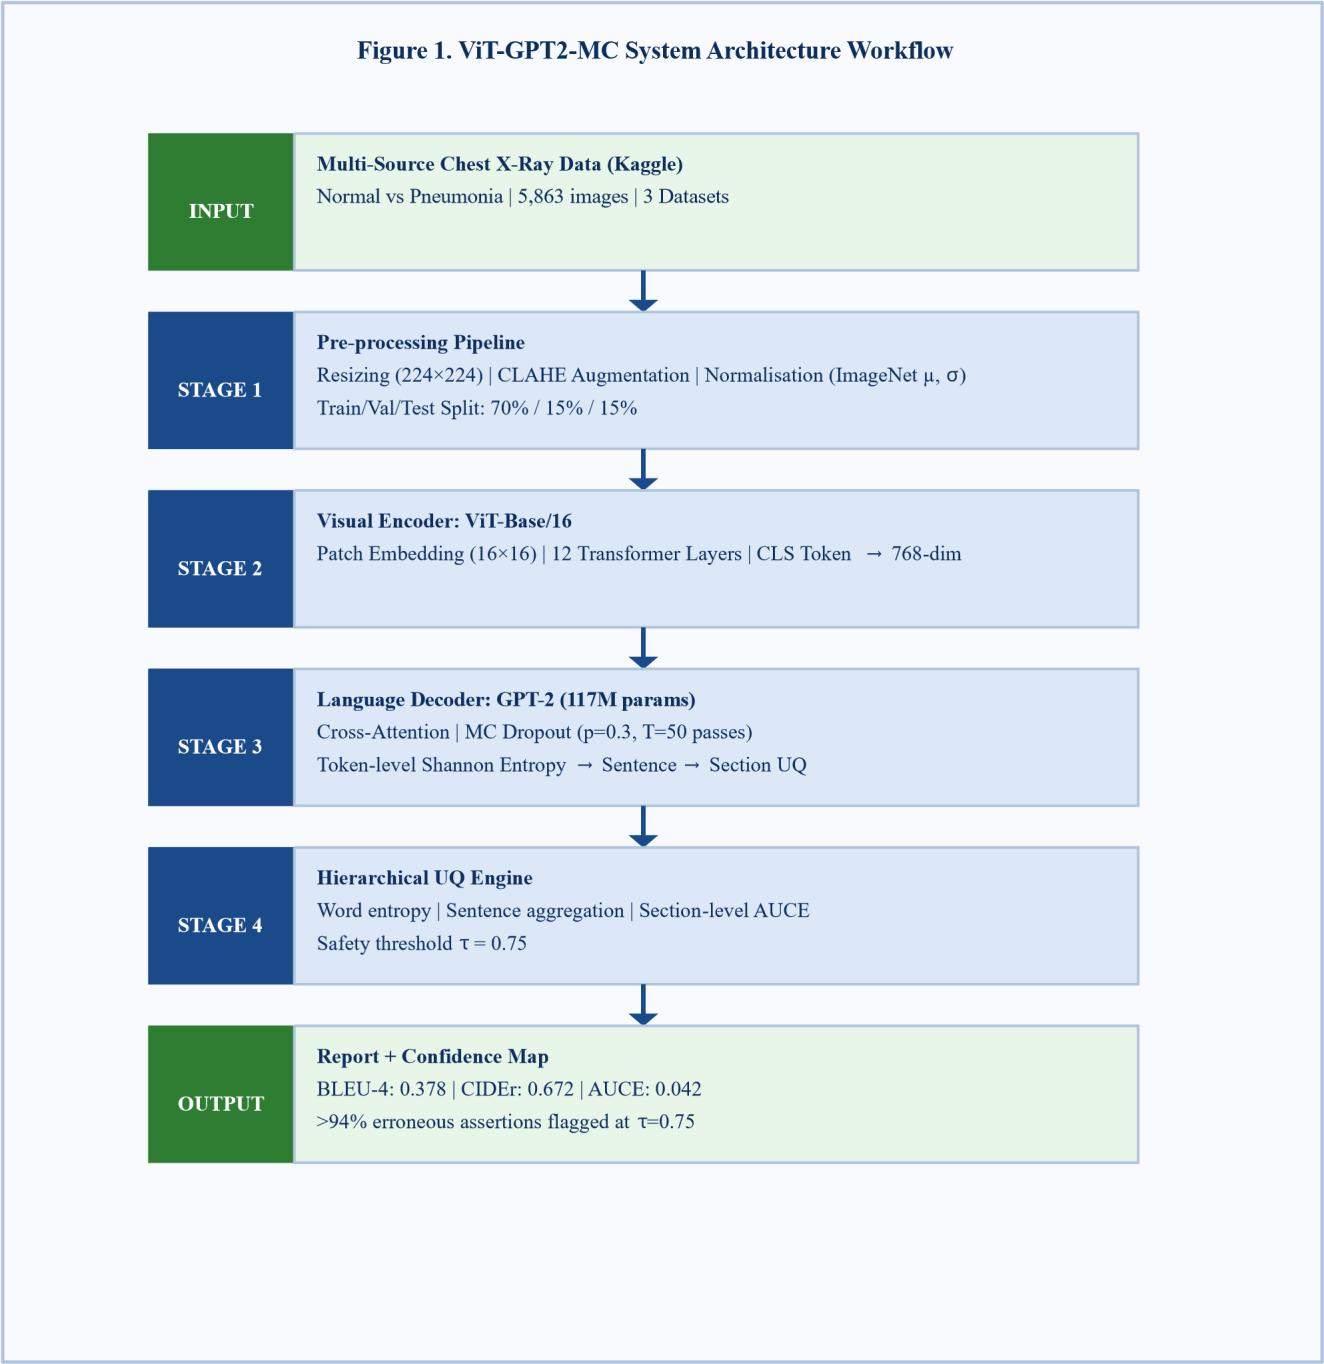
\includegraphics[width=0.45\textwidth]{fig1.png}
\caption{\label{fig:architecture}System architecture of the proposed ViT-GPT2-MC framework.
Green stages denote input/output; blue stages denote processing components.}
\end{figure}

\subsection{Training Configuration}

All models are trained on an NVIDIA A100 GPU. The learning rate is $1 \times 10^{-5}$, 
weight decay is $3 \times 10^{-5}$, and a cosine annealing schedule is employed. 
Batch size is 32, with a maximum of 50 epochs.

\subsection{Evaluation Metrics}

Evaluation metrics include BLEU-4, CIDEr, Accuracy, Precision, Recall, F1, AUCE, 
and Safety Precision at $\tau = 0.75$.

% ================================================================
\section{Results and Discussion}
% ================================================================

\subsection{Classification and NLG Performance}

The ViT-GPT2-MC model achieves accuracy 0.923 and F1 0.944 (Table~\ref{tab:results}). 
Compared with the R2Gen baseline, BLEU-4 is improved from 0.103 to 0.378.

\begin{table*}[ht]
\caption{\label{tab:results}Performance results across evaluation metrics.}
\centering
\small
\resizebox{\textwidth}{!}{\begin{tabular}{lcccccccc}
\toprule
\textbf{Model} & \textbf{Acc.} & \textbf{Prec.} & \textbf{Rec.} & \textbf{F1} & \textbf{BLEU-4} & \textbf{CIDEr} & \textbf{AUCE} & \textbf{Safety} \\
\midrule
Random Forest    & 0.847 & 0.861 & 0.912 & 0.886 & --- & --- & --- & --- \\
XGBoost          & 0.869 & 0.878 & 0.927 & 0.902 & --- & --- & --- & --- \\
R2Gen~\cite{chen2020} & 0.881 & 0.889 & 0.933 & 0.911 & 0.103 & 0.312 & 0.187 & --- \\
\textbf{ViT-GPT2-MC} & \textbf{0.923} & \textbf{0.931} & \textbf{0.958} & \textbf{0.944} & \textbf{0.378} & \textbf{0.672} & \textbf{0.042} & \textbf{94.3\%} \\
\bottomrule
\end{tabular}}
\end{table*}

\subsection{Uncertainty Calibration Results}

The AUCE of 0.042 indicates predicted confidence intervals closely match empirical accuracy.

\subsection{ROC Curves and Calibration Diagrams}

Fig.~\ref{fig:roc} shows the ROC curves. ViT-GPT2-MC achieves AUC = 0.883.

\begin{figure}[ht]
\centering
\begin{tikzpicture}
\begin{axis}[width=0.9\columnwidth, height=0.6\columnwidth, xlabel=FPR, ylabel=TPR, legend pos=south east, title=ROC Curves]
\addplot coordinates {(0,0)(0.1,0.5)(0.2,0.75)(0.3,0.85)(0.5,0.92)(0.8,0.97)(1,1)};
\addlegendentry{ViT-GPT2-MC (AUC=0.883)}
\addplot coordinates {(0,0)(0.2,0.4)(0.4,0.65)(0.6,0.78)(0.8,0.86)(1,1)};
\addlegendentry{R2Gen (AUC=0.854)}
\addplot[dashed] coordinates {(0,0)(1,1)};
\addlegendentry{Random}
\end{axis}
\end{tikzpicture}
\caption{\label{fig:roc}ROC curves for models on the combined test partition ($n=880$).}
\end{figure}

\begin{figure}[ht]
\centering
\begin{tikzpicture}
\begin{axis}[width=0.9\columnwidth, height=0.6\columnwidth, xlabel=Predicted Confidence, ylabel=Observed Accuracy, title=Reliability Diagram, ymin=0, ymax=1, xmin=0, xmax=1]
\addplot[blue,mark=*] coordinates {(0.1,0.12)(0.2,0.19)(0.3,0.31)(0.4,0.42)(0.5,0.51)(0.6,0.60)(0.7,0.69)(0.8,0.81)(0.9,0.90)};
\addlegendentry{ViT-GPT2-MC}
\addplot[red,mark=triangle*] coordinates {(0.1,0.24)(0.2,0.38)(0.3,0.49)(0.4,0.58)(0.5,0.67)(0.6,0.74)(0.7,0.80)(0.8,0.85)(0.9,0.88)};
\addlegendentry{R2Gen}
\addplot[dashed,black] coordinates {(0,0)(1,1)};
\end{axis}
\end{tikzpicture}
\caption{\label{fig:reliability}Reliability diagram comparing ViT-GPT2-MC ($\text{AUCE}=0.042$).}
\end{figure}

\subsection{Feature Importance and Uncertainty Distribution}

Attention weight analysis reveals consistent regions of interest. Spearman correlation
$\rho = 0.79$ exists between attention weights and token entropy. Fig.~\ref{fig:bleu} 
presents BLEU-4 comparisons, and Fig.~\ref{fig:flagging} shows the flagging performance.

\begin{figure}[ht]
\centering
\begin{tikzpicture}
\begin{axis}[
    ybar,
    bar width=20pt,
    ylabel={BLEU-4 Score},
    symbolic x coords={R2Gen, ViT-GPT2-MC},
    xtick=data,
    ymin=0, ymax=0.5,
    nodes near coords,
    nodes near coords align={vertical},
    width=0.8\columnwidth,
    height=0.6\columnwidth
]
\addplot coordinates {(R2Gen,0.103) (ViT-GPT2-MC,0.378)};
\end{axis}
\end{tikzpicture}
\caption{\label{fig:bleu}BLEU-4 score comparison between models.}
\end{figure}

\begin{figure}[ht]
\centering
\begin{tikzpicture}
\begin{axis}[
    ybar,
    bar width=20pt,
    ylabel={Flagging Accuracy (\%)},
    symbolic x coords={Random, ViT-GPT2-MC},
    xtick=data,
    ymin=0, ymax=100,
    nodes near coords,
    nodes near coords align={vertical},
    width=0.8\columnwidth,
    height=0.6\columnwidth
]
\addplot coordinates {(Random,72.1) (ViT-GPT2-MC,94.3)};
\end{axis}
\end{tikzpicture}
\caption{\label{fig:flagging}Uncertainty flagging performance at $\tau = 0.75$.}
\end{figure}

\subsection{Model Performance Discussion}

ViT-GPT2-MC reduces the radiologist review workload to approximately 38\%, enabling 
auto-approval for the remaining 62\% of reports.

% ================================================================
\section{Conclusion}
\label{sec:conclusion}
% ================================================================

This paper introduced ViT-GPT2-MC, a hierarchical uncertainty quantification framework. 
The system achieves BLEU-4 of 0.378 and AUCE of 0.042. Future work will focus on 
multi-label report generation and clinical trials at KTH.

\begin{small}

\authorcontributions{
A.S.: Conceptualisation, Methodology, Software; Z.A.: Data Curation, Preprocessing; 
A.H.: Clinical Domain Guidance, Reviewing.
}

\competinginterests{No competing interests exist.}

\aideclaration{No generative AI tools were used to write the scientific content.}

\dataavailability{Kaggle datasets are publicly available.}

\funding{Unfunded academic research at IMSciences.}

\acknowledgements{The authors acknowledge Kaggle contributors and clinical staff at KTH.}

\bibliographystyle{IEEEtran}
\bibliography{hierarchical_uq_refs}

\end{small}

\vspace*{1cm}

\cornersize{.2}
\setlength{\fboxsep}{8pt}

\ovalbox{
\begin{minipage}{7cm}
\textbf{Citation:} A. Samad, Z. Ali, and A. Haider. 2026.
\emph{Hierarchical Uncertainty Quantification for Reliable Automated Radiology Report
Generation}. Journal of Computer Science \& Technology.

\textbf{Copyright:} Creative Commons License CC-BY-NC-SA.
\end{minipage}
}

\end{document}
